\graphicspath{{./figures/}}

The following section provides details in the construction of the model for predicting stock prices, as well as a description of the ARIMA model to which we compare the network.

\section{ARIMA}
To fit an ARIMA model we need to first perform some basic data exploration to identify key features in the time series. Our aim is to attempt to identify the order of the model through observations of the plots instead of relying on innefficient but exhaustive grid search. 

In total, there are three model parameters we need to identify:
\begin{itemize}[nosep]
    \item[-] $p$, autoregressive terms
    \item[-] $d$, integrated terms
    \item[-] $q$, moving average terms
\end{itemize}%

We begin by plotting autocorrelation functions for the entire dataset and each stock individually. Slow degradation of the ACF plot tends to point to autoregressive terms while the opposite is true for moving average terms. Figure \ref{tab:smallACF} shows us the autocorrelation plot for all the stocks. We observe a slow fall in the ACF plot, which is consistent with autoregressive terms in the model.

\begin{figure}[H]
    \centering
    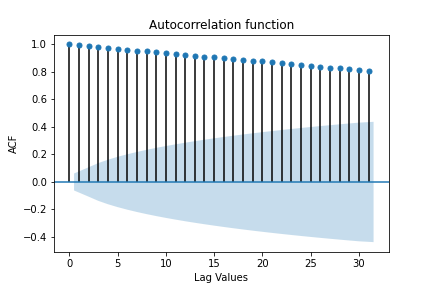
\includegraphics[scale=0.7]{smallACF.png}
    \caption{Autocorrelation function before any differencing}
    \label{tab:smallACF}    
\end{figure}

This graph also tells us that there is significant correlation in the series for over 30 lags. No differencing has been done at this point, the strong correlation could be caused by autocorrelation at lags 1 or 2, which is confirmed by the Partial Autocorrelation function plot below:

\begin{figure}[H]
    \centering
    \begin{subfigure}{.5\textwidth}
        \centering
        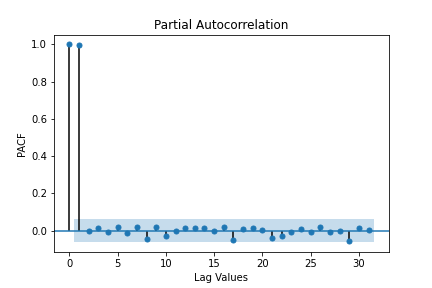
\includegraphics[scale=0.6]{PACF.png}
        \label{tab:PACF}        
    \end{subfigure}%
    \begin{subfigure}{.5\textwidth}
        \centering
        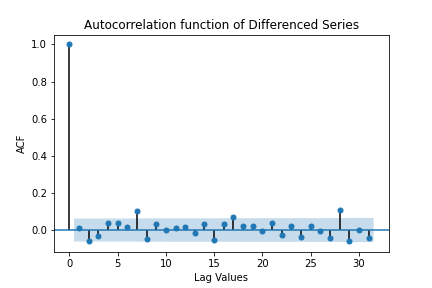
\includegraphics[scale=0.6]{ACFDifferenced.png}
        \label{tab:differenced}
    \end{subfigure}
    \caption{PACF and ACF of differenced series}
\end{figure}

We observe two significant spikes at lags 1 and 2, indicating that the series needs to be differenced twice, $d = 2$. We also observe a major positive spike at $lag=1$ for the differenced ACF plot on the right, which suggests we should add another autoregressive term.

We conclude that a good estimate on the hyperparameters of the ARIMA model we are going to use would be (2, 2, 0), for 2 autoregressive terms, 2 differencing terms and 0 moving average terms.

Using the \texttt{statsmodel} Python module, we create and validate our ARIMA model using walk-forward validation:

\begin{figure}[H]
    \begin{minted}[mathescape, linenos, numbersep=5pt, gobble=2, frame=lines, framesep=2mm]{python}
        train, test = X[:train_size], X[train_size:]
        predictions = []
        for t, _ in enumerate(test):
            model = ARIMA(train, order=(2,2,0))
            model_fit = model.fit(disp=False)
            yhat = model_fit.forecast()[0]
            predictions.append(yhat)
            train.append(test[t])

        mse = mean_squared_error(test, predictions)
        mae = mean_absolute_error(test, predictions)
    \end{minted}
    \caption{Walk Forward Validation of ARIMA model using the \texttt{statsmodels} library}
    \label{code:arima}
\end{figure}

A training and testing split of 80-20 was used to evaluate ARIMA, the same split we use to evaluate the neural network approach.

\section{LSTM}
The network is a relatively simple network by most accounts, comprised of a single hidden layer. The simplicity of the model only goes to show the power of neural networks in fitting and forecasting time-series. The model consists of three layers, an input layer, a Long Short-Term Memory (LSTM) layer and the output layer, as shown in \ref{tab:model_arch}.

\begin{figure}[H]
    \centering
    \begin{neuralnetwork}[height=4]
        \newcommand{\x}[2]{$x_#2$}
        \newcommand{\y}[2]{$\hat{y}_#2$}
        \newcommand{\h}[2]{$h_#2$}
        \newcommand{\hlast}[2]{\ifnum4=#2 \vdots \else \ifnum5=#2 $h_{100}$ \else $h_#2$ \fi \fi}
        \inputlayer[count=4, bias=false, title=Input, text=\x]
        \hiddenlayer[count=5, bias=false, title=LSTM, text=\hlast] 
        \linklayers
        \hiddenlayer[count=1, bias=false, title=Dense, text=\h]
        \linklayers
        \outputlayer[count=1, title=Output, text=\y] 
        \linklayers
    \end{neuralnetwork}
    \caption{Model Architecture}
    \label{tab:model_arch}
\end{figure}

The input layer receives a 2-dimensional array of historical stock values, including the previous day's opening, highest, lowest and closing stock prices. The network then allows the neurons to compete amongst each other and determing an appropriate output. Output is in the shape of a 1-dimensional array containing four values, the future day's predicted stock values for open, high, low and close. The LSTM layer contains 100 nodes and is trained for 100 epochs. The Rectifier Linear Unit was used as its activation function and the Mean Absolute Error was used as its loss function.

\begin{table}[H]
    \centering
    \begin{tabular}{|r|r|l|r|l|l|}
        \hline
        \textbf{Nodes} & \textbf{Epochs} & \textbf{Optimizer} & \textbf{Learning Rate} & \textbf{Activation} & \textbf{Loss} \\ \hline
        100            & 100             & Adam               & 0.001                  & ReLU                & MAE           \\ \hline
        \end{tabular}
    \caption{Description of the hidden LSTM layer}
    \label{tab:lstm_layer}
\end{table}

In this project we made use of the Keras API to implement the network. Keras is written in Python and operates ontop of TensorFlow, which is an extremely popular and widely used Deep Learning library\citesuper{chollet2015keras}. A simple sequential model using LSTM cells built using Keras would look like this:

\begin{minted}[mathescape, linenos, numbersep=5pt, gobble=2, frame=lines, framesep=2mm]{python}
    model = Sequential()
    model.add(LSTM(100, activation="relu", input_shape=(n_steps, n_features)))
    model.add(Dense(n_features))
    opt = Adam(learning_rate=0.001)
    model.compile(optimizer=opt, loss="mae", metrics=["mse"])
\end{minted}

With as little as 5 lines of code, we have a working Long Short-Term Memory model ready for training. The LSTM cell easily remembers the long term dependencies in the data and outputs a 1-dimensional array containing future values. Figure \ref{tab:layer_description} contains a more detailed breakdown of the layers used in the network.

\begin{figure}[H]
    \centering
    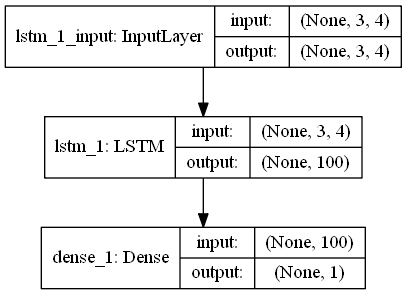
\includegraphics[width=80mm]{model_plot}
    \caption{Description of layers}
    \label{tab:layer_description}
\end{figure}

A Dense layer is a fully-connected feedforward layer. Feedforward layers are the simplest type of architecture employed in machine learning, which is essentially a collection of neurons that pass signals in one direction only, the layer in front of them. These layers do not form cycles in their connections which is fundamentally different from Recurrent Neural Networks like the LSTM. The purpose of the Dense layer in the model is to reduce the dimensionality of the data from the 100-dimensional space created in the LSTM down to a 1-dimensional array of values, which is then lead to the output layer. The Dense layer performs no operations on the data, it's activation function is linear.

\section{Model Evaluation}
To perform an evaluation of the model, we feed into it the testing set gathered from the dataset. The model uses the Mean Absolute Error metric to guide the minimisation of its loss function during training. Mathematically, the Mean Absolute Error is defined as

\begin{align}
    \text{MAE} = \frac{1}{n} \sum\limits_{i=1}^{n} {|\hat{y_i} - y_i|}
\end{align}

and is the sum of the absolute differences of predicted data points to actual data points divided by the number of data points in the set. MAE is also used in the evaluation of the compiled and trained model.

Evaluation of the model also includes a comparison of Mean Squared Error values. MSE is mathematically defined as

\begin{align}
    \text{MSE} = \frac{1}{n} \sum\limits_{i=1}^{n} {(\hat{y_i} - y_i)^2}    
\end{align}

and is the mean of the squared differences between the predicted values and the actual data points. MAE was chosen for the training of the model because of its linear relationship between penalties and errors, in that it treats a predicted to actual difference of 1 in a way proportionally to how it treats a predicted to actual difference of 5. MSE treats larger differences between predictions and actual data non-linearly. 

\begin{figure}[H]
    \centering
    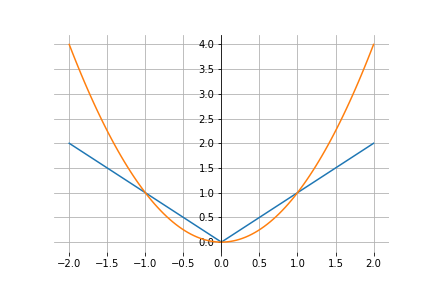
\includegraphics[width=100mm]{maevsmse}
    \caption{Comparison of MAE (blue) and MSE (orange). Note how MAE scales linearly with higher error values while MSE scales quadratically, treating higher errors more harshly.}
    \label{tab:maevsmse}
\end{figure}